\documentclass{article}
\usepackage{graphicx}
\usepackage{tikz}
\usepackage[paperwidth=3.5in, paperheight=5in, margin=0in]{geometry}
\pagestyle{empty}

\begin{document}
\begin{figure*}
    \centering
    \begin{tikzpicture}
    \node[anchor=south west,inner sep=0] (image) at (0,0) {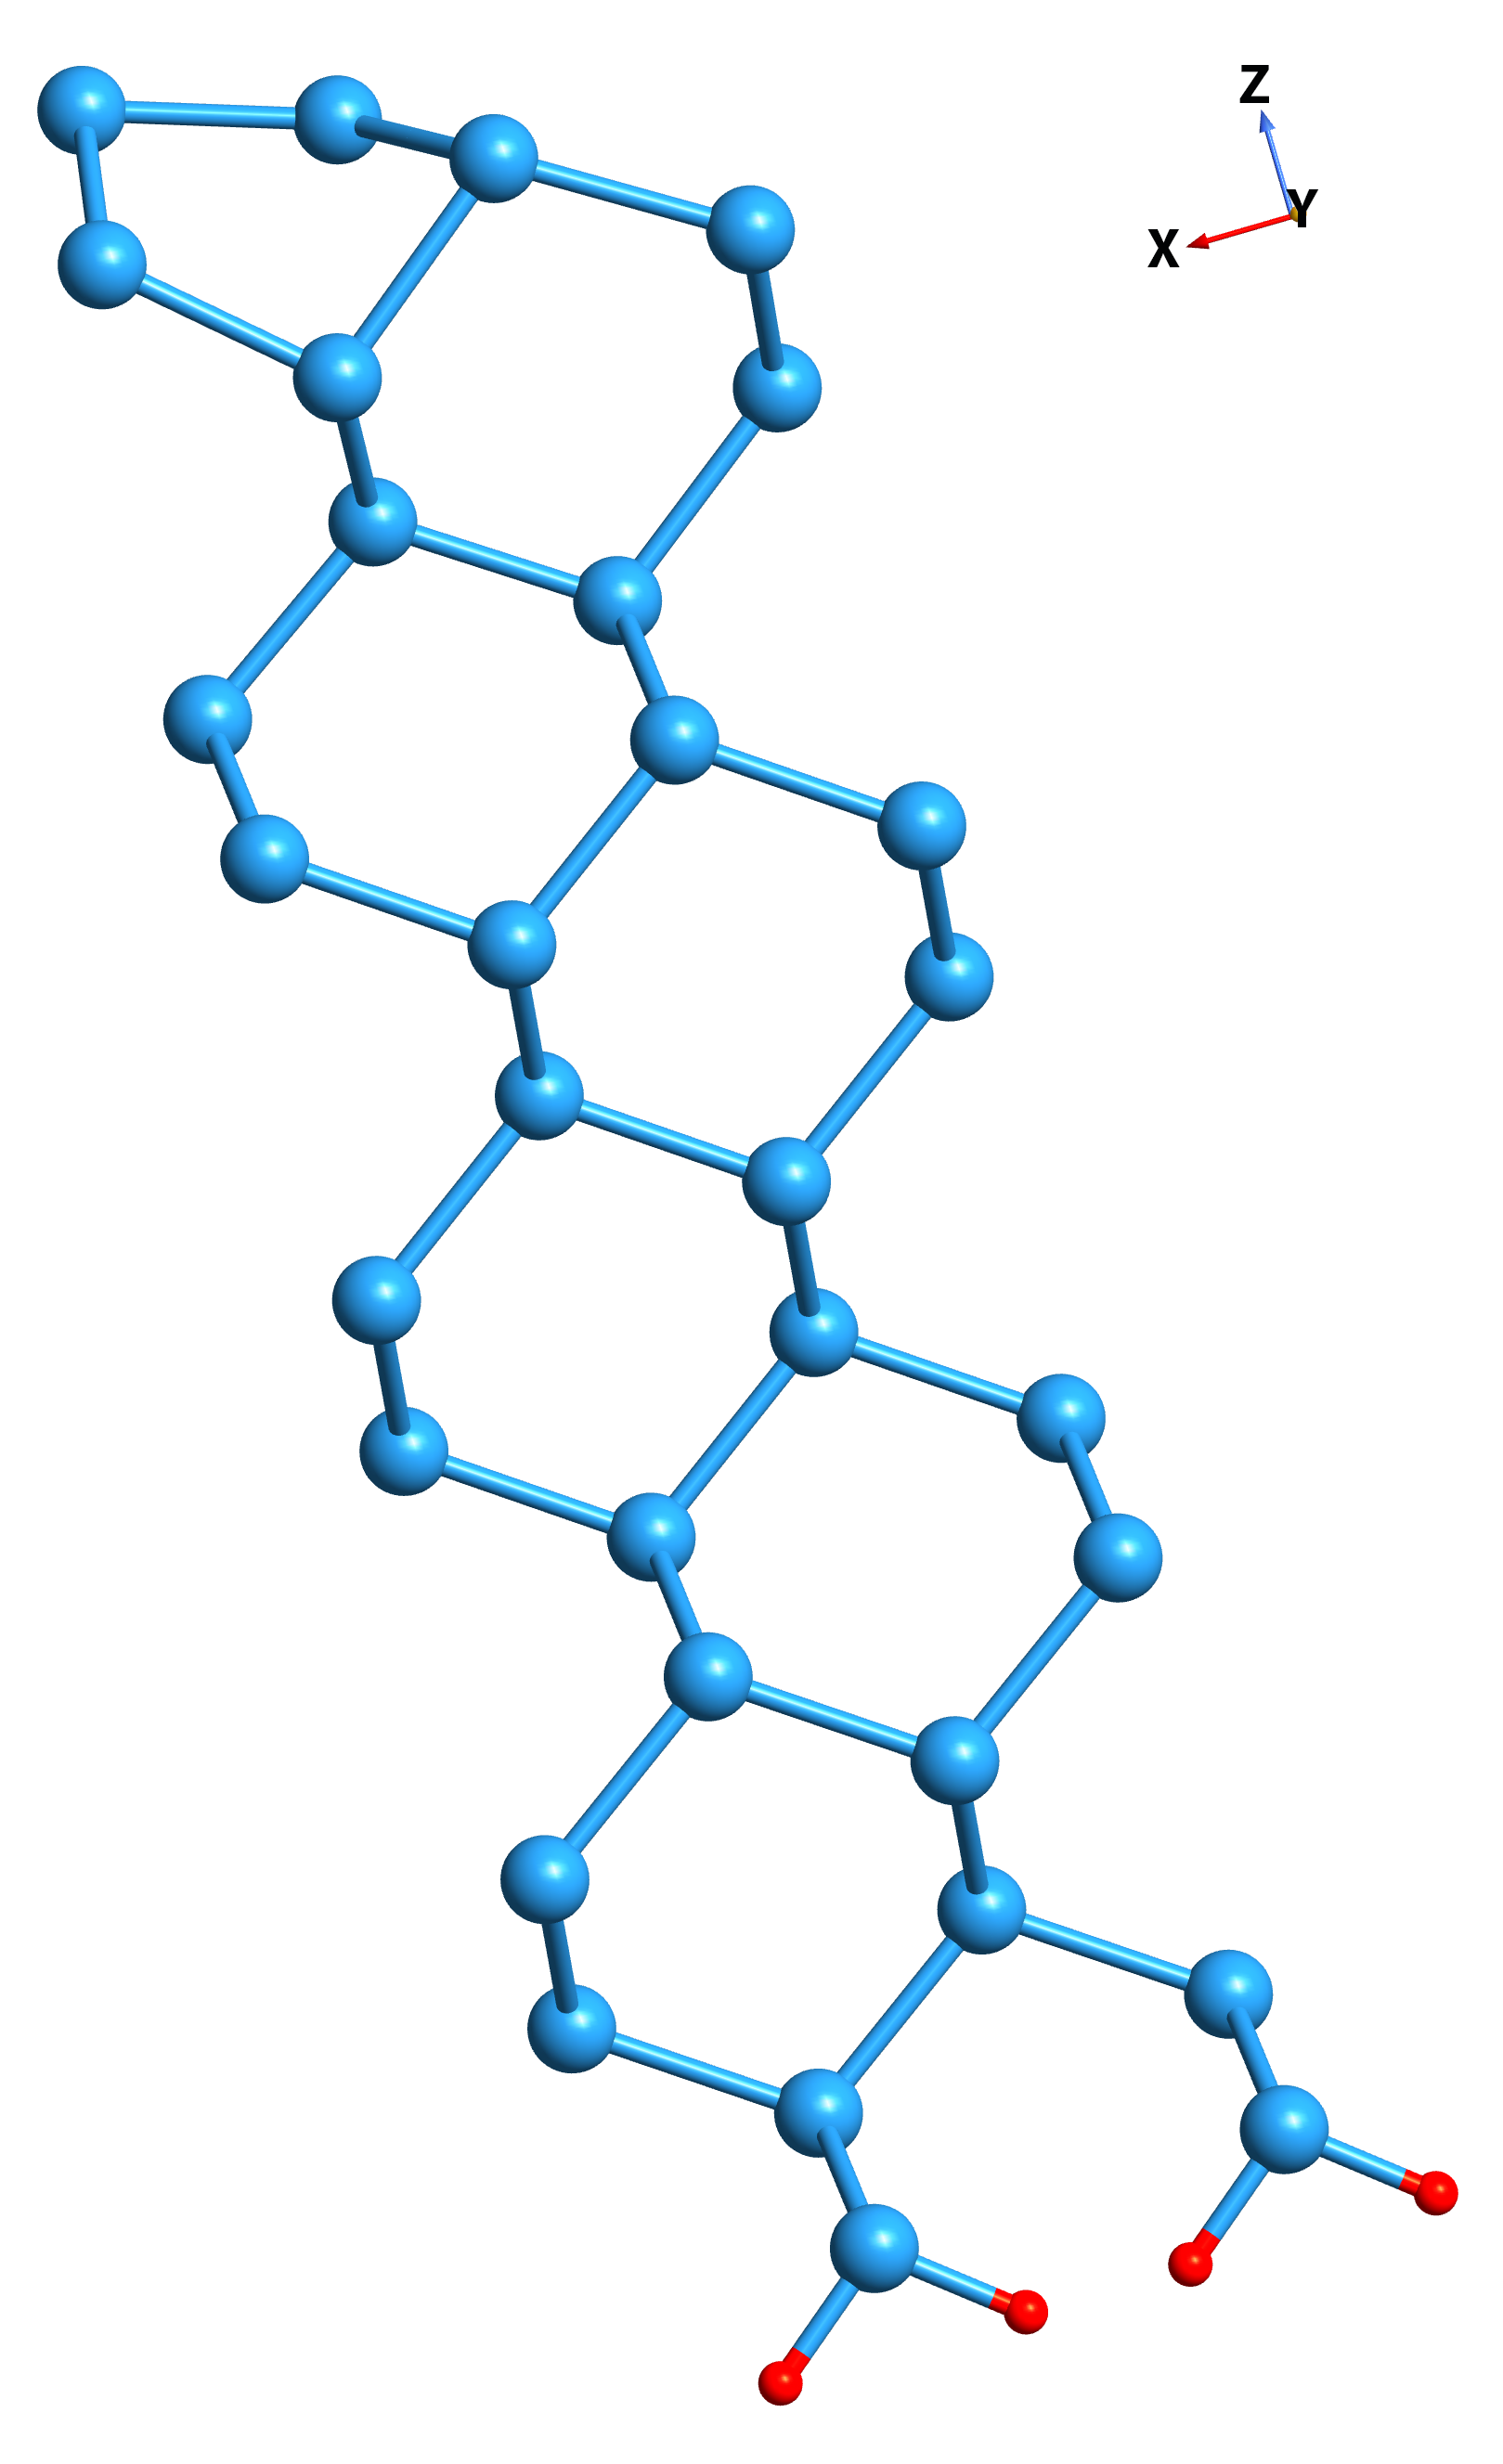
\includegraphics[width=0.75\textwidth]{Si2x1-rot}};
    \begin{scope}[x={(image.south east)}, y={(image.north west)}]
        \node at (0.5,1.04) {2$\times$1 reconstruction $\Rightarrow\chi^{xxx}_{\mathrm{2\times 1}}\ne 0$};
        \node[rotate=15.5] at (0.82,0.57) {${\mathcal{C}}^{\ell}(z) = 1$};
        \draw[color=red, thick, dashed] (0,0.40) -- (1,0.57);
        \node[rotate=15.5] at (0.85,0.51) {${\mathcal{C}}^{\ell}(z) = 0$};
        \node at (0.5,-0.03) {H-terminated $\Rightarrow\chi^{xxx}_{\mathrm{H}}= 0$};
    \end{scope}
    \end{tikzpicture}
\end{figure*}
\end{document}
